\subsection{Characterization of Performance}

\subsubsection{Experiment Design}

We illustrate the high throughput capabilities of the HTBAC workflow using
ESMACS protocol by examining scalability in the number of pipelines and
characterizing the performance of the workload. We also demonstrate that the
absolute performance of the workload is unrelated to the scalability of
Ensemble Toolkit.

The amount of replicas required by ESMACS has an upper-bound of 25 replicas
yet we extend the number replicas to 128 in order to demonstrate higher
scalability with a greater degree of confidence for the potential HTBAC user.

\subsubsection{Experiment Setup}

We perform scalability experiments on Blue Waters HPC resource-- a 13.3
petaFLOPS Cray at NCSA and University of Illinois, with 32 Interlago cores/50
GB RAM per node, Cray Gemini, Lustre shared file system.

We validate the performance of the runtime system, RADICAL-Pilot, using weak
scalability to to demonstrate that RP can schedule tasks concurrently,
provided that sufficient resources are available. We characterize the weak
scalability of the ESMACS protocol using Ensemble Toolkit running exclusively
on Blue Waters CPUs. In the pilot description of EnTK, the pilot size is
contingent upon characterization of performance i.e. weak or strong scaling.
In the event of weak scaling we provide the same number of cores in the pilot
size description as the number of cores required by the workload. The number
of cores is varied between 64-1024 while hte number of simulations is kept
equal to the number of cores at all times. For example, in the ESMACS
protocol, the simulation task specifies 8 cores per pipeline, therefore the
pilot size is defined as 8 $\times$ number of pipelines. We vary the number
of pipelines to characterize weak scaling performance where the tasks are
scheduled concurrently. For each of these configurations, the simulation
execution time is observed to be constant.

In order to demonstrate that RP is invariant to the type of workload we run
two types of experiments: We ran the HTBAC workflow with null workload in
which each task did no work (/bin/sleep 0), the actual simulation workload.
The size of the workload is varied in proportion to the amount of resources
such that all tasks are concurrently executed at all times. We range the
number of replicas ranged from 8 to 128 running concurrently using either 1
or 8 cores per replica, depending on the task. All the experiments use
Ensemble Toolkit version 0.47 and RADICAL-Pilot version 0.42.

In the MD workload, the simulation tasks are executed using NAMD-MPI. The
equilibration stages 4 and 6 are assigned 5000 timesteps while stage 5
requires 55000 timesteps.

\subsubsection{Results}

We perform weak scalability characterization of HTBAC for both null workload
and NAMD workload by measuring the overhead introduced by RP and the total
time to completion (TTC).

% The RP overhead demonstrates the core overhead which is the
% time-to-completion (TTC) as measured by RADICAL Pilot as well as the Blue
% Waters file system overhead, network communication, time to stage the
% units, and the latency of communication to the database.

% For the NAMD workload, we show weak scaling results for the overheads and
% the simulation execution time which corresponds to the time taken by all
% the simulations to complete.

\begin{figure}[!htbp]
  \centering
  \begin{minipage}[b]{0.49\textwidth}
  \centering
  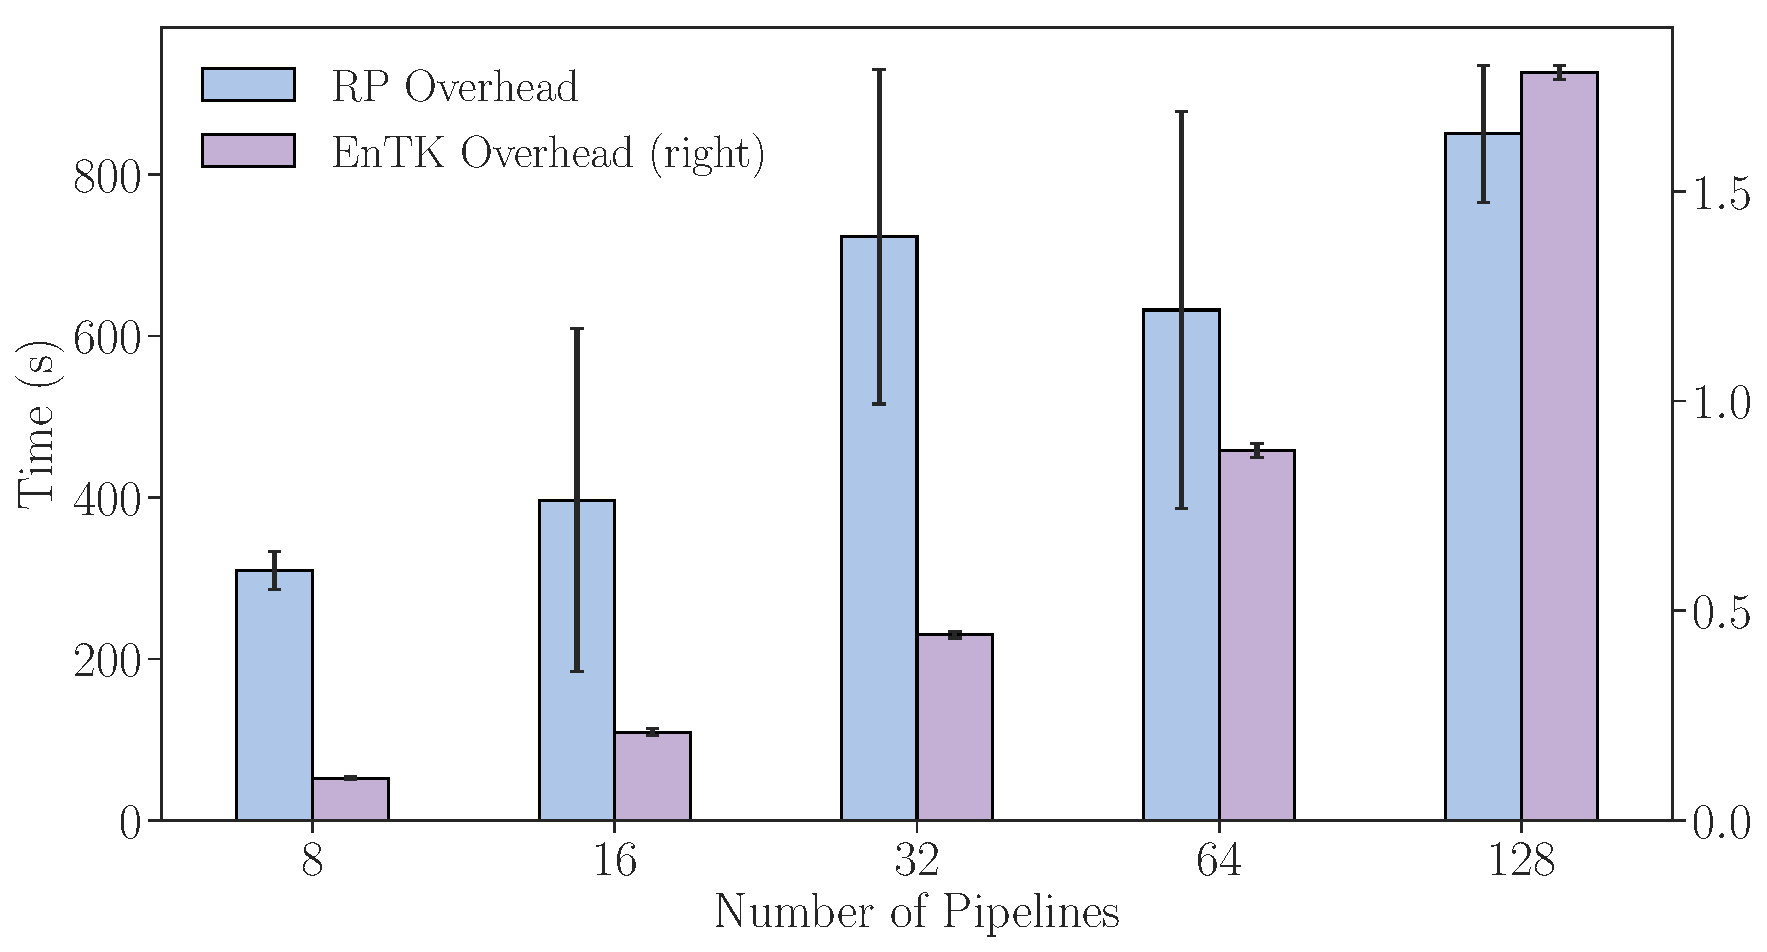
\includegraphics[width=\textwidth]{FIGURES/null_workload_overheads.pdf}
  \end{minipage}
  \begin{minipage}[b]{0.49\textwidth}
  \centering
  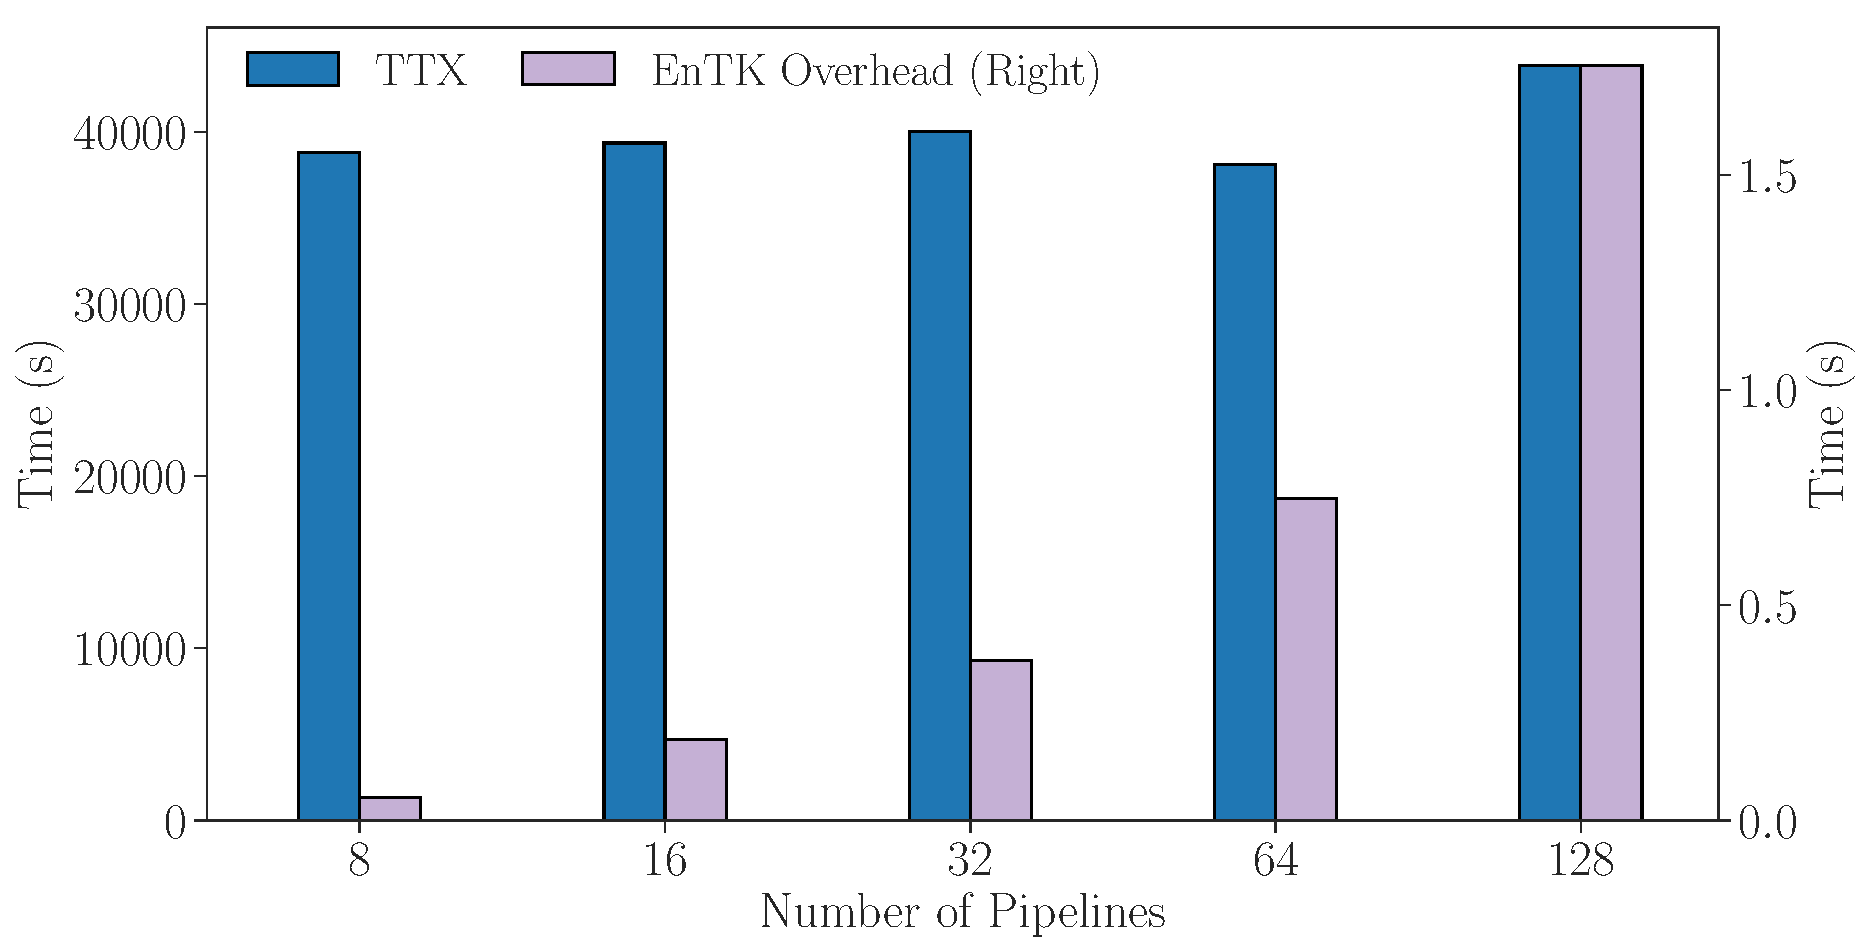
\includegraphics[width=\textwidth]{FIGURES/namd_workload_overheads.pdf}
  \end{minipage}
  \caption{\textbf{Top:} Weak scaling of HTBAC using null workload. We
          observe similar behavior at each configuration in the simulation
          execution time showing that the RADICAL-Pilot is invariant to the
          workload and a steady increase in the RP overhead due to the
          increase in the number of stages. \textbf{Bottom:} Weak scaling of
          HTBAC using NAMD workload. We observe higher simulation execution
          times than the null workload yet similar behavior in all NAMD
          configurations.}\label{fig:htbac_perf}
\end{figure}


The fluctuation of the simulation execution times can be attributed to
run-time system fluctuations within the workload including stragglers at
higher pipeline and pipeline-to-pipeline fluctuations. In order to examine
the fluctuations within stages we corrolate the overhead for each pipeline at
the longest simulation duration in order to reconcile any fluctuations
induced by NAMD\@. We calculate time-to-execution (Tx) of the largest
pipeline size and compare the longest MD run within each pipeline. The NAMD
logs indicate a mean and variance as\ldots

\begin{figure}[!htbp]
  \centering
  %\begin{minipage}[b]{0.6\textwidth}
  \begin{minipage}[b]{0.55\textwidth}
  \centering
  %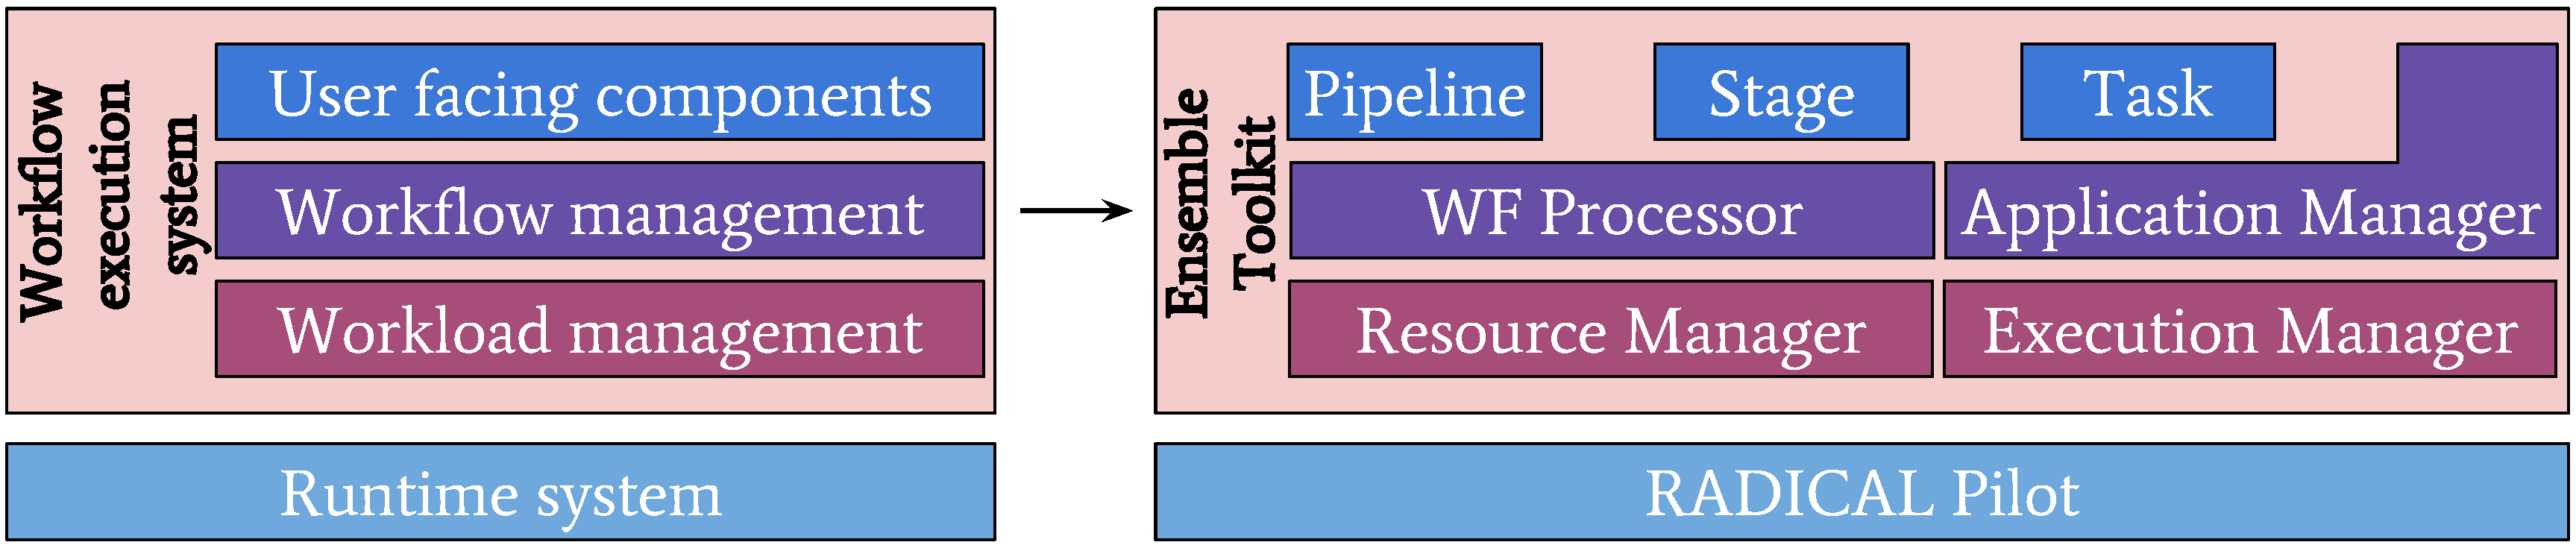
\includegraphics[width=\textwidth, height=35mm]{FIGURES/entk_overview.pdf}
%  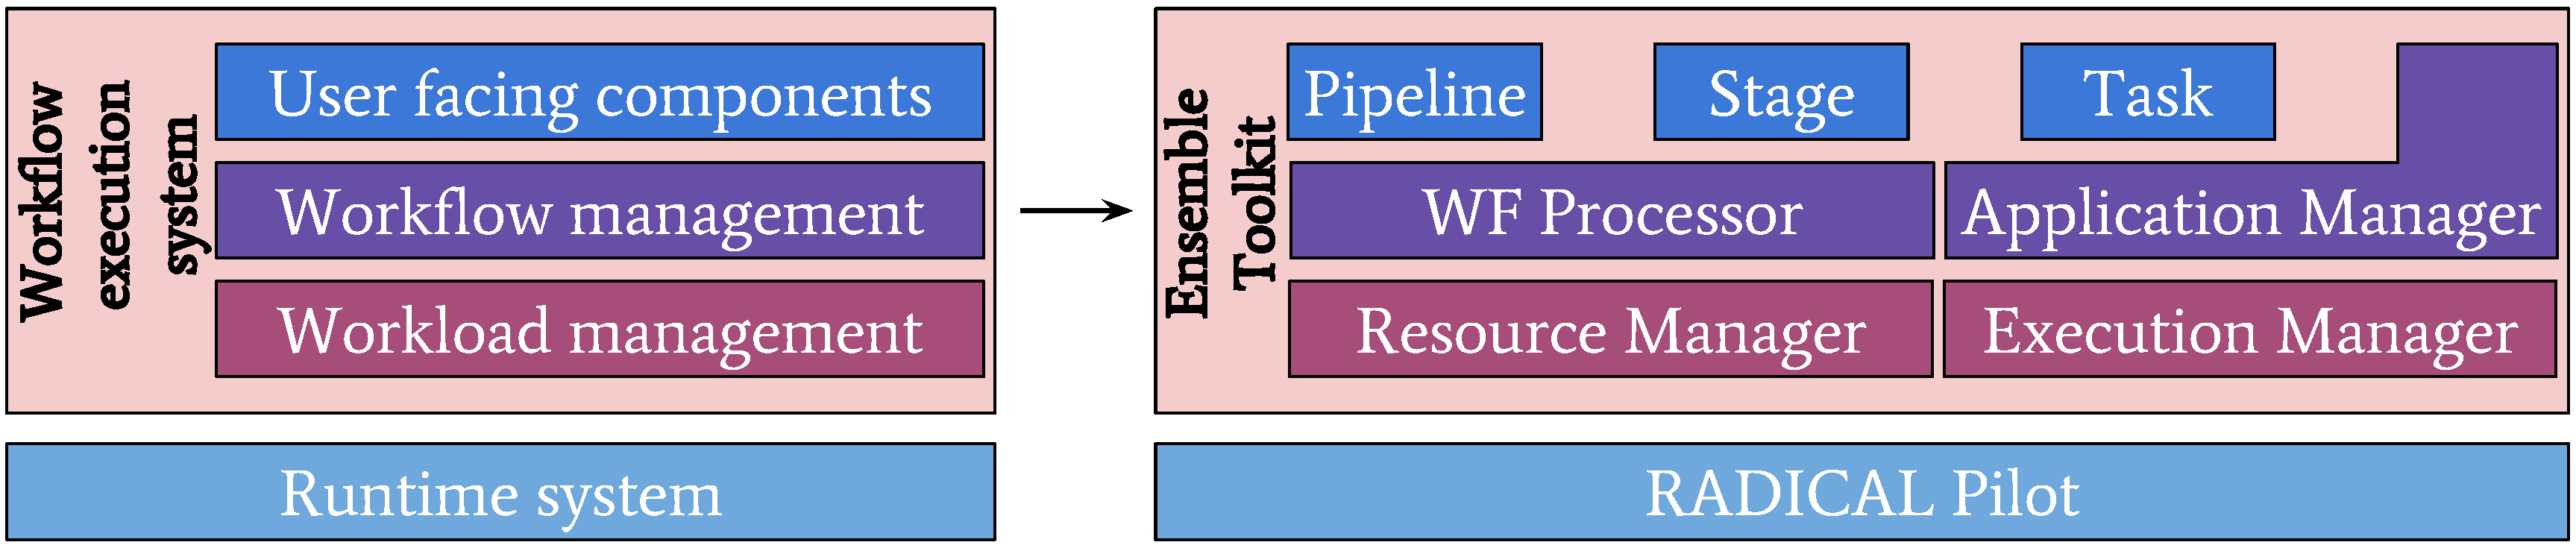
\includegraphics[width=\textwidth, height=40mm]{FIGURES/entk_overview.pdf}
  \end{minipage}
  %\begin{minipage}[b]{0.39\textwidth}
  \begin{minipage}[b]{0.44\textwidth}
  \centering
%  \includegraphics[width=\textwidth, height=35mm]{FIGURES/md_general.pdf}
%  \includegraphics[width=\textwidth, height=40mm]{FIGURES/md_general.pdf}
  \end{minipage}
  \caption{Overview of time-to-execution (Tx) of each pipeline at the
           longest simulation duration as measured by NAMD log files, showing
           how the distribution shows no abnormal fluctuations across
           pipelines.}\label{fig:namd_logs}
\end{figure}

%NAMD logs - corrolate the overhead for each pipeline makes the system invariant to the worload. Remaining will be RP overhead. NAMD log files (utime) demonstrates time-to-execution (Tx) 

%Add in: what are the overheads, how is EnTK collecting overhead 




%eq0 : Minimize with decreasing restraints
%eq1 : NVT, 50K, with restraints
%eq2 : NPT, 300K, with decreasing restraints 
%sim1.conf: NPT, 300k, no constraints


Need system verification of timestamps (errors) 




